\runningheader{Oppgave a)}{}{Side \thepage\ av \numpages}

\item[]   Alle modellene i denne delen av øvingen skal implementeres
  i subsystemet\\
  \fbox{\tt Om Integrator-blokken, oppgave 2a)-2e)} i 
  skallfilen \fbox{\tt oving2.slx}, og alle modellene skal 
  benytte integratorblokken som numeriske integrerer
  et  inngangssignal $u(t)$ i henhold til
  \begin{equation}
    \label{eq:8}
  y(t) = \int_{0}^{t} u(\tau) d\tau + y(0)
\end{equation}
hvor $y(0)$ er initialverdien.
Vær klar over at alle signalene vi jobber med er
diskrete som $\{u_{k}\}$, men at vi for enkelhets skyld skriver
signalene som kontinuerlige som $u(t)$.



  
% ********************************************************
% oppgave a) 
% ********************************************************
\item


  I denne deloppgaven er $u(t)$ en konstant, og du skal relatere
  simuleringsresultatet til integralregning fra matematikken.
  Implementer modellen vist under.
  \begin{figure}[H]
    \centering
    \hspace*{0mm}\scalebox{0.8}{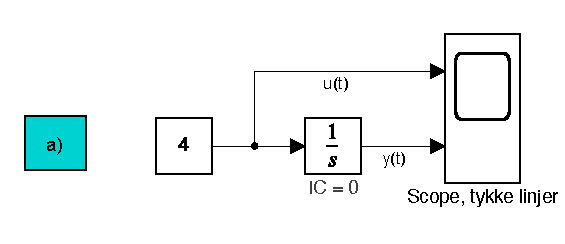
\includegraphics{2a.pdf}}
  \end{figure}
  Utgangen fra {\sf  Constant}-blokken 
  er $u(t)$ og utgangen fra {\sf  Integrator}-blokken
  er  $y(t)$. La  initialverdien til integratorblokken være
  $y(0){=}0$.   {\color{red}La simuleringstiden være 25 sekund.}

  
{\bf Svar på følgende spørsmål:    }
  \begin{enumerate}[label=a\arabic*)]
  \item  Bruk ligning~\eqref{eq:8} og  la $u(t){=}4$. Hva blir det
    matematiske uttrykket for $y(t)$ når $y(0){=}0$?  

  \item  Bruk det matematiske uttrykket til å beregne verdien av $y(t)$ ved
     tidspunkt  $t{=}25$~sekund.
  
   \item Simuler modellen og svar samtidig på følgende spørsmål:
     ``Stemmer simulerings\-resultatet med svaret du fant i  forrige
     delspørsmål?''

     Ta med simulerings\-resultatet i
     innleveringen ved bruke prosedyren på
     side~\pageref{page:prosedyre}.
     
\item  Endre initialverdien til $y(0){=}10$ og simuler. Hvordan endres
  det matematiske uttrykket til $y(t)$? Vis at 
  simuleringsresultatet overstemmer med det matematiske uttrykket. Ta
  med figur i innleveringen.

\end{enumerate}
